\section{Overview of the Evaluation Strategy}
Counterfactuals were evaluated using both AI-based metrics and human evaluation.

\section{AI-Based Quantitative Evaluation}

\subsection{Evaluating the VAE Reconstruction Performance}
traditional loss like MSE loss vs logcosh loss comparison.
The SSIM and PSNR scores were computed to measure the quality of image reconstructions.
A visualization of reconstructed vs. original images was analyzed.

To evaluate the quality of the counterfactual explanations generated by our three methods: 
\textbf{Grid-Based Masking, LIME on Images, LIME on Latent Features}, we collected user ratings based on three criteria: 
\textbf{Interpretability, Plausibility, Visual Coherence}. Users rated each counterfactual on a scale of 1 (poor) to 5 (excellent). 
The collected data were stored in a CSV file, and we computed the mean ratings for each method and criterion.


\subsection{Counterfactual Success Rate (CSR) Across Different Masking Methods}
CSR measures how often a counterfactual successfully flips the classifier’s decision.
Comparison of CSR across different masking methods:
LIME on Latent Features: X%
Grid-Based Masking: Y%
Object Detection-Based Masking: Z%
LIME on Images: W%


\subsection{Structural and Visual Quality of Counterfactuals}
SSIM and PSNR were computed for counterfactual images to assess realism.






\section{Human Evaluation of Counterfactual Explanations} \label{section:Human Evaluation of Counterfactual Explanations}

\subsection{Study Setup and Procedure}
Participants were presented with counterfactual images generated by different masking techniques.
They were asked to select the most preferred counterfactual explanation based on:
Interpretability
Plausibility
Visual Coherence

\subsection{User Preferences for Different Masking Methods}
Percentage of participants preferring each method was analyzed.


\subsection{Correlation Between Human Preferences and AI-Based Metrics}
The relationship between human-selected best counterfactuals and AI-based evaluation scores (CSR, SSIM, PSNR) was analyzed.


\

\subsection{Quantitative Analysis}
\label{subsec:quantitative_analysis}

Our design aligns with insights from Delaney et al.~\cite{DELANEY2023103995}, who argue that evaluation of counterfactuals should reflect human explanation goals. They show that traditional metrics like L1/L2 distance are often misaligned with human expectations of plausibility. Accordingly, we incorporate both quantitative metrics validity and a human rating study focused on interpretability, Plausibility, and Visual Coherence and semantic consistency.

Figure~\ref{fig:barPlotAll} shows a combined bar chart comparing average ratings for Interpretability, Plausibility, and Visual Coherence 
across the three counterfactual methods. Meanwhile, Figure~\ref{fig:heatmap} provides a heatmap visualization for these metrics, 
making it easy to compare each method's performance at a glance.

\begin{figure}[htbp]
    \centering
    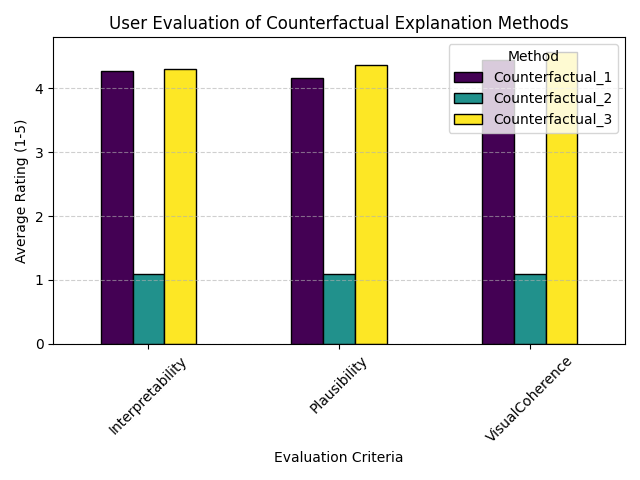
\includegraphics[width=0.7\textwidth]{img/results/bar_plot_user_evaluations.png}
    \caption{User Evaluation of Counterfactual Explanation Methods: Combined Bar Chart}
    \label{fig:barPlotAll}
\end{figure}

\begin{figure}[htbp]
    \centering
    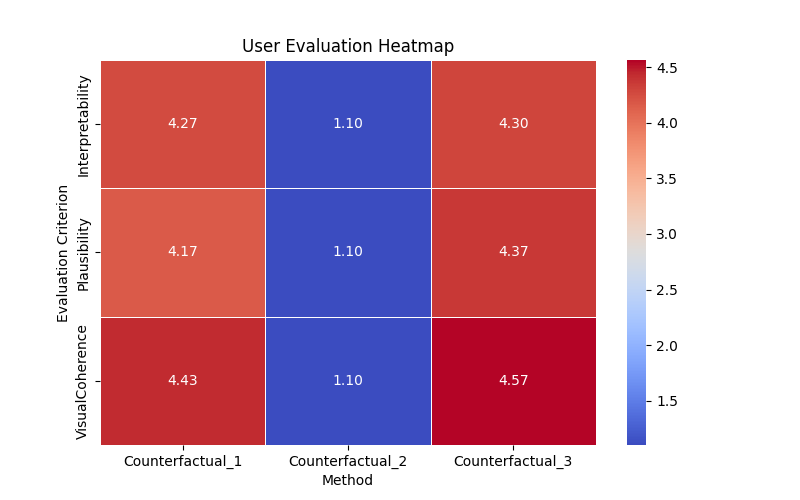
\includegraphics[width=0.7\textwidth]{img/results/heatmap_user_evaluations.png}
    \caption{User Evaluation Heatmap for Three Counterfactual Methods}
    \label{fig:heatmap}
\end{figure}

In addition to these combined views, we generated individual bar charts for each criterion (Figures~\ref{fig:interpretabilityBar}, 
\ref{fig:plausibilityBar}, and \ref{fig:visualCoherenceBar}). Each figure focuses on one metric and plots the average rating 
for each counterfactual method.

\begin{figure}[htbp]
    \centering
    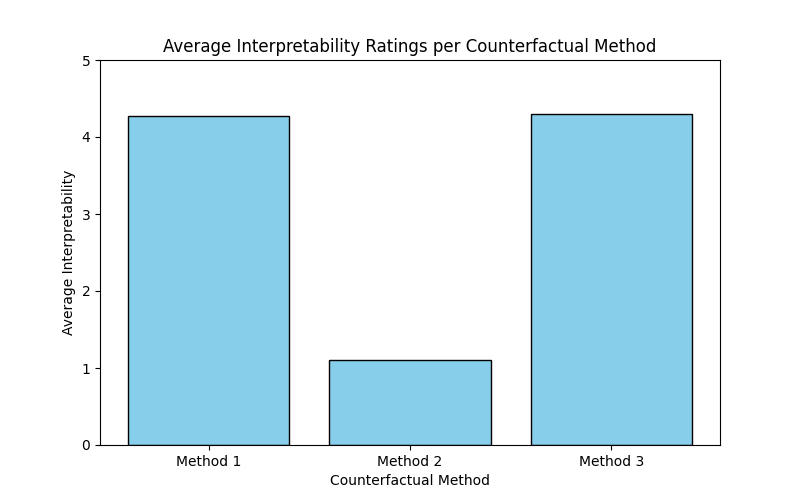
\includegraphics[width=0.55\textwidth]{img/results/Interpretability_ratings.png}
    \caption{Average Interpretability Ratings per Counterfactual Method}
    \label{fig:interpretabilityBar}
\end{figure}

\begin{figure}[htbp]
    \centering
    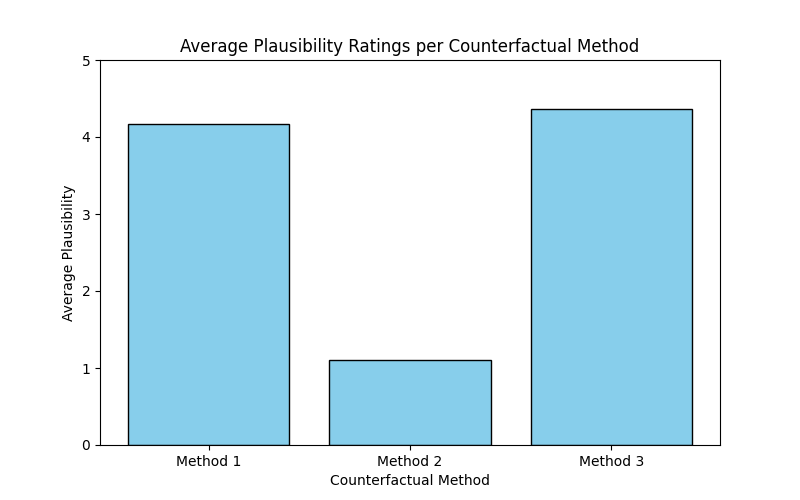
\includegraphics[width=0.55\textwidth]{img/results/Plausibility_ratings.png}
    \caption{Average Plausibility Ratings per Counterfactual Method}
    \label{fig:plausibilityBar}
\end{figure}

\begin{figure}[htbp]
    \centering
    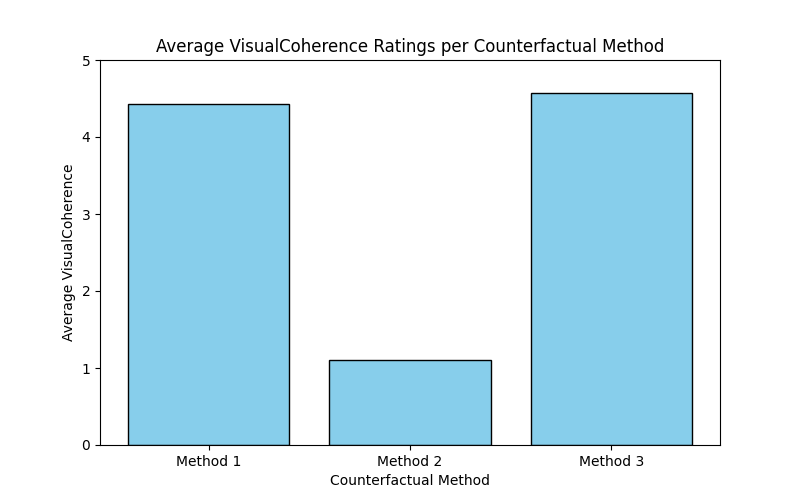
\includegraphics[width=0.55\textwidth]{img/results/VisualCoherence_ratings.png}
    \caption{Average Visual Coherence Ratings per Counterfactual Method}
    \label{fig:visualCoherenceBar}
\end{figure}

Overall, these visualizations indicate that \textbf{Method 3} achieves the highest scores across most metrics, particularly in 
\textit{Visual Coherence} and \textit{Interpretability}, while \textbf{Method 2} often lags behind in \textit{Plausibility} and 
\textit{Visual Coherence}. \textbf{Method 1} offers moderate-to-high performance in most categories but does not surpass Method 3.

\section{Validity}
\label{sec:validity}
Validity is a measure of how often the counterfactual explanation is successfully generated. 
The validity percentage is computed as
\[
\text{Validity (\%)} = \left( \frac{\text{Successful Counterfactuals}}{\text{Total Counterfactuals}} \right) \times 100.
\]

For our methods, a counterfactual is considered valid if it changes the model’s predic-
tion to the desired target class (e.g., from STOP to GO, or from RIGHT to LEFT). 

Table~\ref{tab:validity_results} summarizes the validity results obtained from four different methods:

\begin{table}[htbp]
    \centering
    \caption{Validity of Counterfactual Explanations}
    \label{tab:validity_results}
    \begin{tabular}{lcccc}
        \hline
        \textbf{Method} & \textbf{Total} & \textbf{Successful} & \textbf{Validity (\%)} \\
        & \textbf{Counterfactuals} & \textbf{Counterfactuals} & \\
        \hline
        Grid-Based Masking & 2326 & 2316 & 99.57 \\
        Object Detection & 2326 & 84 & 3.61 \\
        LIME on Images & 2326 & 2044 & 87.88 \\
        LIME on Latent Features & 2326 & 211 & 9.07 \\
        \hline
    \end{tabular}
\end{table}

As seen in Table~\ref{tab:validity_results}, the Grid-Based Masking approach achieved a very high validity of 99.57\%, meaning that nearly all counterfactuals generated by this method were successful. In contrast, the Object Detection method and LIME on Latent Features produced much lower validity values (3.61\% and 9.07\% respectively), indicating that these methods struggled to consistently generate valid counterfactual explanations. LIME on Images yielded a moderately high validity of 87.88\%, suggesting that while it generally succeeds, it does not match the near-perfect performance of Grid-Based Masking.

These findings suggest that the Grid-Based Masking approach is the most robust in generating counterfactual explanations under the conditions tested, while Object Detection and LIME on Latent Features require further refinement to improve their consistency.

\section{Interpretability}
\label{sec:interpretability}
Interpretability refers to the ability to explain or provide the meaning of a system in terms understandable to humans. In our study, 
participants rated each counterfactual on how clear and direct it was in showing \emph{what changed} to alter the AI's decision. 
As shown in Figures~\ref{fig:barPlotAll} and~\ref{fig:interpretabilityBar}, Method 3 obtained the highest average interpretability score.

\section{Plausibility}
\label{sec:plausibility}
Plausibility checks whether the modified (counterfactual) image still looks like a realistic driving scene. If the alterations 
(e.g., removing a pedestrian or adding a turn signal) appear unnatural, the user perceives the explanation as less plausible. 
In Figure~\ref{fig:plausibilityBar}, Method 3 again led in plausibility, while Method 2 often produced blurred or otherwise 
unrealistic modifications, leading to lower user scores.

\section{Visual Coherence}
\label{sec:visualcoherence}
Visual Coherence asks if only the relevant parts of the image are changed while the rest of the scene remains intact. 
This helps isolate the effect of a single element (such as a fallen branch or an oncoming car) on the AI's decision. 
Method 3 excelled here as well, as depicted in Figures~\ref{fig:barPlotAll} and~\ref{fig:visualCoherenceBar}, suggesting 
it can more precisely localize the critical regions in the image.

\subsection{Overall Discussion}
These results suggest that Method 3’s approach to generating counterfactual explanations is most effective at preserving 
scene realism (\textbf{plausibility}) and focusing changes on only the necessary parts (\textbf{visual coherence}) while 
still being easy for users to understand (\textbf{interpretability}). The detailed user feedback and comments support 
these quantitative findings, with many noting that Method 2’s modifications were often “blurred” or “very bad image,” 
explaining its low scores.

Overall, these ratings confirm that focusing on targeted changes and realistic reconstructions significantly enhances 
user perception of counterfactual explanations, an insight that can guide further refinement of deep generative models 
in autonomous driving contexts.